%!TEX root = ../thesis.tex
\chapter{Blockchain}
\label{blockchain}

A \textit{blockchain} is a \textit{distributed transaction ledger}~\cite{nakamoto2012bitcoin}. It consists of a continuously growing list of \textit{blocks} which are linked, ordered, and immutable. Each block typically contains a \textit{hash pointer} being a link to a previous block, a timestamp and a list of \textit{transactions}. Transactions describe the transfer of assets from one entity to another. A distributed network is formed by the users of the system without central control. Each node of the network contains a local copy of the blockchain; the transaction ledger. To come to an agreement on the correct ledger, the network uses a decentralized \textit{consensus} mechanism with which integrity is achieved and malicious activity is prevented.

Blockchains are potentially suitable for financial activities, the recording of events, medical records~\cite{blockchain_ehr,Azaria2016}, and other record management activities, such as identity management, transaction processing or documenting provenance. Blockchain can be seen as a distributed immutable, tamper-proof, and audit log that records all data transactions. As a result any attempt to tamper blockchain is immediately evident and easily detectable.

\textit{Bitcoin}~\cite{nakamoto2012bitcoin} is the first decentralized \textit{cryptocurrency}, a monetary system without central authority invented by an unknown person or a group of people under the name of \textit{Satoshi Nakamoto}~\cite{nakamoto2012bitcoin}. Its ability to provide a solution to the \textit{double spending problem}~\cite{double_spent, nakamoto2012bitcoin} made it a powerful digital currency among physical currencies in less that 10 years, triggering an explosion of more than 800 other digital coins.

The goal of this chapter is to present of the basic operating principles of the blockchain, which are based on the foundation of cryptography -- without getting to unnecessary details or rigorous mathematical proofs. As Bitcoin was the first decentralized blockchain system that put the bases for others to be made and involve~\cite{7163021,10.1007/978-3-662-46803-6_10, ethereum_whitepaper}, we mainly focus on blockchain internals. Notable variations of blockchains that support features of our interest are mentioned selectively further in this chapter.

\section{History}\label{blockchain:history}

Credit card transactions are the dominant payment method that is used on the web today~\cite{Narayanan:2016:BCT:2994437}. This system is handled by a financial
system involving processors, banks, credit card companies and other intermediaries. Normally a credit card transaction is realized as follows: first, the buyer sends over his credit card details to the merchant; then the merchant sends and validates the data in the financial system.

Buyers may not want to handle their credit card details to an unknown vendor over an insecure channel. Intermediate services -- such as Paypal -- sits between the buyer and the seller and the intermediate service approves
the transaction and notify the seller. This allows the buyer to keep his anonymity and avoid security risks.

The idea of \textit{digital cash} was first introduced by David Chaum in his paper~\cite{Chaum1983}, entitled ``Blind Signatures for Untraceable Payments'', in 1983. In 1990 Chaum proposed the first off-line e-cash system~\cite{Chaum:1988:UEC:646753.704915} and founded DigiCash~\cite{chaum1983blind}, an electronic money corporation that sent the first electronic payment in 1994.

Digital cash schemes are vulnerable to that is called double-spending~\cite{10.1007/978-3-662-46803-6_10, 7163021}. It comes up when the same digital token is spent more than once.  Chaum found a way to both keep the system anonymous and prevent double-spendings with the use of \textit{blind signatures}~\cite{Chaum1983,Chaum:1988:UEC:646753.704915}.
Yet still, Chaum's solution needed a centralized trusted oracle which validated the transactions. Many cryptographers attempted to improve Chaum's scheme over the years. Okamoto and Ohta~\cite{Watanabe1996}, for example, in 1996 implemented coin subdivisions with the use of \textit{Merkle trees}~\cite{merkle_tree}.

About the same time, a group of cryptographers called \textit{Cypherpunks}~\cite{cypherpunk,cypherpunks_manifesto} was formed and advocate the widespread
use of strong cryptography and privacy-enhancing technologies~\cite{cypherpunks_manifesto} as a way to social and political change. Cypherpunks electronic mailing list, through which they communicating originally, was the predecessor to the mailing list where Satoshi Nakamoto would announce later Bitcoin~\cite{nakamoto2012bitcoin}. Chaum's ideas are supposed to have set the technical roots of the vision of the Cypherpunk movement~\cite{cypherpunk}. Chaum patented the blind-signature scheme preventing others from developing ecash system that use the same protocol. Violating Chaum's patents, Cypherpunks implemented an e-cash system called Magic Money~\cite{magic_money} which further developed his technology.

However, DigiCash failed to gain public attraction. Its main problem was that  banks and merchants would not adopt it for commercial and financial purposes.

In 1991, Haber et al.~\cite{Haber1991} proposed a scheme for \textit{secure timestamping} of digital documents using digital signatures and hash pointers in previous documents, thus creating a chain of document certificates. In an improvement which was proposed later documents were collected into a block, all the blocks linked together in a chain. This data structure form of the skeleton for Bitcoin's blockchain.

A year later, cryptographers Dwork and Naor came up with a solution to email spamming~\cite{Dwork1993} by using \textit{computational puzzles}.They created the idea of \textit{Proof-of-Work}. In 1997, Adam Back proposed a similar idea that he called Hashcash~\cite{hash_cash}. Back's Proof-of-Work system set the basis for Bitcoin's consensus mechanism.

Wei Dai at 1998 proposed b-money~\cite{b_money}, an anonymous distributed electronic cash system, in which everyone could create money using a Proof-of-Work mechanism like Ηashcash. B-money used the notion of a secured timestamp ledger as used by Haber et al. for digital documents~\cite{Haber1991}.

In 2008, Satoshi Nakamoto published a paper under the title \textit{``Bitcoin: A Peer-to-Peer Electronic Cash System''} on The Cryptography Mailing list at metzdowd.com~\cite{satoshi_mailing_list} describing the Bitcoin protocol. The Bitcoin network came into existence on 3 January 2009 with the release of the first Bitcoin client, \verb|wxBitcoin|, and the issuance of the first Bitcoins~\cite{btc_client, btc_first_block}. Bitcoin represents a decade long work of research in cryptography combining several prior inventions~\cite{antonopoulos2014mastering}.

Bitcoin is the first decentralized digital currency. The Bitcoin network is a fully distributed peer-to-peer network that anyone can freely join by running an open source implementation of the bitcoin protocol. Bitcoin does not rely on a trusted central authority and was he first applied solution to overcome the \textit{Byzantine Generals' Problem}~\cite{byzantine_fault_tolerance}. Bitcoin makes use a Proof-of-Work consensus mechanism that keeps  the public ledger consistent, prevents double-spends and confirms transactions. It can also be used to achieve consensus on decentralized networks for elections, lotteries, asset registries, and more~\cite{antonopoulos2014mastering}.

Running from 2009, Bitcoin is the most well studied Blockchain network~\cite{10.1007/978-3-662-46803-6_10} with various published papers on different topics such as privacy~\cite{10.1007/978-3-319-70278-0_8, 10.1007/978-3-642-39884-1_2, Bonneau14e.w.:mixcoin, 10.1007/978-3-662-44774-1_9}, economics~\cite{Babaioff:2012:BRB:2229012.2229022, 10.1007/978-3-319-70278-0_17, Bentov2017DecentralizedPM, Carlsten:2016:IBW:2976749.2978408}, attacks~\cite{DBLP:journals_corr_Bahack13, DBLP:journals_corr_EyalS13}, network~\cite{10.1007/978-3-662-44774-1_7, 190890} and scalability~\cite{kiayias2017non, 10.1007/978-3-662-53357-4_5, 10.1007/978-3-662-53357-4_8}. Over the years, Bitcoin's blockchain has grown significantly is size making it difficult for certain devices to store all of it and run as a full node. Specifically, In April 2018 the Bitcoin's blockchain size is over 160GB~\cite{btc_bl_size}.

Bitcoin does not scale efficiently. There is a limit on the amount of transactions the bitcoin network can process. The maximum transaction processing capacity is estimated between 3.3 and 7 transactions per second~\cite{10.1007/978-3-662-53357-4_8}. The limit is related to the block size limit -- the total number of transactions a block can contain -- that was introduced as an anti-spam measure. Various solutions proposed to address this issue. One implemented solution is \textit{Segregated Witness} (SegWit, BIP 141)~\cite{segwit}. The SegWit implementation increased the block size by a factor of approximately of two.

\section{Identity}\label{blockchain:identity}

In Bitcoin, and in most cryptocurrencies, there is no inherent notion of \textit{identities} or individual accounts which ``own'' coins~\cite{7163021,nakamoto2012bitcoin}. There is no users, account balance or identities—these all exist only to the extent that they can be imputed from the list of published transactions~\cite{7163021,nakamoto2012bitcoin}.

Identity is defined as a cryptographic key pair $(s_k, p_k)$, where $s_k$ is the private key and $p_k$ the public key. The private key is used for spending a ``coin'' and the public key as the address of the user. No real-world name or identifying information are required~\cite{7163021,nakamoto2012bitcoin}.

In Bitcoin, due to the public nature of the blockchain it is sometimes possible to trace the flow of money between public keys (\textit{addresses}) and conclude that they are likely controlled by the same
individual~\cite{7163021,10.1007/978-3-319-17016-9_1}. For that reason, Bitcoin's identity system is considered \textit{pseudonymous}. The underlaying non-anonymous Internet infrastructure (nodes leak their IP address when broadcasting transactions),
together with the availability of all bitcoin transactions in the blockchain, has proven to be an anonymity threat~\cite{10.1007/978-3-319-17016-9_1, 7163021,Meiklejohn:2013:FBC:2504730.2504747,6113303,10.1007/978-3-642-39884-1_2,fi5020237}.
Although Bitcoin provides a limited form of \textit{unlinkability} by letting users create new addresses at any time for any transaction, various techniques, such as transaction graph analysis, can be utilized by an adversary to link together different addresses controlled
by the same entity leading to deanonimity~\cite{7163021,Meiklejohn:2013:FBC:2504730.2504747,6113303,10.1007/978-3-642-39884-1_2,fi5020237}. Furthermore, Bitcoin does not provide \textit{untraceability} -- for each incoming transaction all possible senders are probable -- since all transactions are public~\cite{cryptonote}.

Altcoins such as Zerocash~\cite{zcash} and CryptoNote~\cite{cryptonote} were focused on improving bitcoin anonymity and integrated unlinkability to their currency proposals. In particular, Zerocash utilize zero-knowledge proofs (zkSNARKs~\cite{10.1007/978-3-642-40084-1_6}) which reveal no information at all about the amount or recipients enabling a completely untraceable ledger. On the other hand, CryptoNote uses \textit{ring signatures} creating a \textit{mixing protocol} satisfying both untraceability and unlinkability. CryptoNote compared to Zerocash has better performance but weaker anonymity~\cite{7163021}.

\section{Network}\label{blockchain:network}

Blockchain networks are \textit{peer-to-peer} networks. Anyone who wants to spend coins can freely join and participate in the network by running a software on their computer. All the nodes of the network are equal. There is no central server or trusted authority, neither hierarchy within the network and both the protocol as well as the software are open. Any blockchain implementation that does not follow that principle should be avoid as is in contrary to the \textit{Kerckhoffs' principle}~\cite{kerckhoffs_principles}.

When a user runs the software it connects to other peers of the network using peer-to-peer discovery schemes. In Bitcoin, there are some nodes called seed nodes, that their IP address is hardcoded in the software, which can be used to quickly discover other nodes. Alternatively, a known IP address of a bitcoin node can be given manually.

\section{Transactions}\label{blockchain:structure:tx}

The basic data structure of the blockchain is a \textit{transaction (tx)} that transfers assets from one party to another. The owner of a coin transfers coins by publishing a digital signature; his desire to perform a transaction that transfers coins to the recipient of the money. By verifying the signature, one can ensure that the sender of the money is truly the one who authorized the transaction. A blockchain transaction can be described as a \textit{node} with two \textit{edges}, one \textit{incoming} edge and one \textit{outcoming} edge~\cite{zindros_thesis}. The incoming edge describes the sender (from) and the outcoming edge the recipient (to). Each edge has the corresponding address of the party; its public key. Every bitcoin transaction has a unique \textit{transaction id (txid)} which is derived by double hashing the transaction with the use of the SHA-256 cryptographic hash function. Payments are done by \textit{linking} transaction nodes and money can be view as a chain of transactions where monetary value pass~\cite{zindros_thesis}. All transactions together form a transaction graph which is public and everyone participating in the network can see and add new transactions to the graph.

\begin{figure}[!ht]
  \centering
  \begin{subfigure}[!ht]{\textwidth}
    \centering
    \begin{tikzpicture}
      \node[tx] (A) at (0,0) {$tx$};
      \draw [->] ++(-3,0) -- (A) node[midway, below]{Alice} node[midway, above]{5mBTC};
      \draw [->] (A) -- ++(3, 0) node[midway, below]{Bob} node[midway, above]{5mBTC};
    \end{tikzpicture}
    \caption{Simplified}
    \label{fig:bl_tx:simple}
    \vspace*{2mm}
  \end{subfigure}
  \begin{subfigure}[!ht]{\textwidth}
    \centering
    \begin{tikzpicture}
      \node[tx] (A) at (0,0) {$tx$};
      \draw [->] (-3,0) -- (A) node[below, xshift=-4.7cm]{\footnotesize{1BvBMSEYstWetqTFn5Au4m4GFg7xJaNVN2}} node[midway, above]{5mBTC};
      \draw [->] (A) -- (3, 0) node[left, below, xshift=1.5cm]{\footnotesize{1J98t1WpEZ73CNmQviecrnyiWrnqRhWNLy}} node[midway, above]{5mBTC};
    \end{tikzpicture}
    \caption{Addresses are public keys}
    \label{fig:bl_tx:pub}
    \vspace*{2mm}
  \end{subfigure}
  \caption{A bitcoin transaction}
  \label{fig:bl_tx:tx}
\end{figure}

\begin{figure}[!ht]
  \centering
  \begin{tikzpicture}
    \node[tx] (A) at (0,0) {$tx$};
    \draw [->] (-3,0) -- (A) node[midway, below]{Alice} node[midway, above]{5mBTC};
    \draw [->] (A) -- (3, 0) node[midway, below]{Bob} node[midway, above]{5mBTC};
    \node (txid) at (-5,0) {$txid = SHA256^{2}($};
    \node (txid) at (3.3,0) {$)$};
  \end{tikzpicture}
  \caption{Bitcoin Transaction ID}
  \label{fig:bl_tx:id}
\end{figure}

When a transaction is made, each node on the network should be able to confirm that the user making the transaction, has indeed the money to transfer. Otherwise, anyone could produce money arbitrarily, sign it and create a valid transaction. As there is no central trusted third party, the whole network have to maintain exactly who has how much coin.

A transaction can have \textit{outgoing unlinked edges}, edges that are not connected to another node transaction. These edges are unspent coins, owned by various users and ready to be spent. This type of edges are called \textit{unspent transaction outputs} (UTXO). The UTXO set, the list of all outgoing unlinked edges, describes how much each user owns and is kept by every node of the network. In this way, the recipient and the network can confirm, by checking the UTXO set, that the sender owns the money at the time of the transaction.

When a user wants to transfer money, first she have to find a transaction that has a UTXO of which she is the owner. Then she creates one transaction with one incoming and one outgoing edge and connect the incoming edge of the new transaction with the old UTXO. Now the old UTXO is not an UTXO anymore, it is just spent, and the outgoing edge of the new transaction is unconnected and becomes the new UTXO. Finally she specifies the value and the owner (address) of the new outgoing edge and signs the transaction. The sign of the transaction is a way of declaring asset ownership. The user have to prove that for a public key -- the address where the UTXO points to -- she holds the corresponding private key. Only the owner of the private key can produce valid signatures that are verifiable under the corresponding public key.

The UTXO set is maintained collectively by the network. When a new full node is connected to the network, the nodes with which it connects inform it about UTXO set and the history of all transactions that occurred from the begging of time. If a full node reconnects after a period on inactivity the node is informed about the new transactions that took place since the last time the node was connected to the network. For the nodes to be able to maintain the UTXO set, the transactions have to be published on the network. This is achieved through a mechanism called broadcasting. When a transaction is created, the participants broadcast the details of the transaction to their neighbours. The neighbours publish the transaction to their neighbours and recursively the transaction is being published until the whole network becomes aware of it.

In Bitcoin there is no notion of giving changes. That is, because there is no accounts with balances and the only way of keeping track money ownership is the UTXO set, the total value of the income edge must be consumed at once. However, a bitcoin transaction can have multiple incoming and outcoming edges. This property is exploited to create a changing system. In particular, when a user wants to transfer money to another user and the value of the UTXO edge is bigger than the desired amount, she can create a transaction with two outcoming edges, one for the recipient and one to give changes to herself.

\begin{figure}[!ht]
  \centering
  \begin{tikzpicture}
    \node[tx] (A) at (0,0) {$tx$};
    \draw [->] (-3,0) -- (A) node[midway, below]{Alice} node[midway, above]{1mBTC};
    \draw [->] (A) -- ++(2, 0) -- ++(1, 1) -- ++(2, 0) node[midway, below]{Bob} node[midway, above]{0.1mBTC};
    \draw [->] (A) -- ++(2, 0) -- ++(1, -1) -- ++(2, 0) node[midway, below]{Alice} node[midway, above]{0.9mBTC};
  \end{tikzpicture}
  \caption{Change exchange}
  \label{fig:bl_tx:change}
\end{figure}

\begin{figure}[!ht]
  \centering
  \begin{tikzpicture}[node distance=3cm]
    \node[tx] (A) at (0,0) {$tx$};
    \node[tx, below of=A] (B) {$tx$};
    \node[tx, below of=B] (C) {$tx$};
    \node[tx, right of=B, node distance=7cm] (D) {$tx$};

    \draw [->] (A) -- ++(4, 0) node[midway, below]{Alice} node[midway, above]{1mBTC} -- (D);
    \draw [->] (B) -- ++(4, 0) node[midway, below]{Alice} node[midway, above]{2mBTC} -- (D);
    \draw [->] (C) -- ++(4, 0) node[midway, below]{Alice} node[midway, above]{1.5mBTC} -- (D);

    \draw [->] (D) -- ++(4, 0) node[midway, below]{Bob} node[midway, above]{4.5mBTC};

  \end{tikzpicture}
  \caption{Transaction multiple inputs}
  \label{fig:bl_tx:change}
\end{figure}

\begin{figure}[!ht]
  \centering
  \begin{tikzpicture}
    \node[tx] (A) at (-5,0) {$tx$};
    \node[tx] (B) at (0,0) {$tx$};
    \draw [->] (A) -- (B) node[midway, below]{Wage} node[midway, above]{1mBTC};
    \draw [->] (B) -- ++(2, 0) -- ++(1, 2) -- ++(2, 0) node[midway, below]{Rent} node[midway, above]{0.6mBTC};
    \draw [->] (B) -- ++(2, 0) -- ++(3, 0) node[midway, below, xshift=1em]{Electricity} node[midway, above, xshift=1em]{0.2mBTC};
    \draw [->] (B) -- ++(2, 0) -- ++(1, -2) -- ++(2, 0) node[midway, below]{Gas} node[midway, above]{0.2mBTC};
  \end{tikzpicture}
  \caption{Transaction multiple outputs}
  \label{fig:bl_tx:multi_out}
\end{figure}

In the Bitcoin transaction graph, the Kirchhoff property mandates that the total outputs of all transactions are at most equal to the total inputs of all transactions. In particular, let $txs$ be all transactions of the network, $out(tx)$ all the output edges of the transaction $tx$, $in(tx)$ all the input edges of the transaction $tx$ and $w(e)$ the value of that edge, it holds that:

\begin{equation*}
  \forall tx \in txs: \sum_{o \in out(tx)}w(o) \leq \sum_{i \in in(tx)}w(i)
\end{equation*}

\begin{figure}[ht!]
    \centering
    \begin{tikzpicture}[scale=0.9]
      \node[tx] (A) at (0,0) {$tx$};
      \node[tx] (B) at (4,0) {$tx$};
      \node[tx] (C) at (8,0) {$tx$};
      \draw [->] (-3,0) -- (A) node[midway, below]{Alice} node[midway, above]{1mBTC};
      \draw [->] (A) -- (B) node[midway, below]{Bob} node[midway, above]{1mBTC};
      \draw [->] (B) -- (C) node[midway, below]{Charlie} node[midway, above]{1mBTC};
      \draw [->] (C) -- (11,0) node[midway, below]{Eve} node[midway, above]{1mBTC};

      \node[red] (D) at (10, 3) {$utxo$};
      \draw [->, red] (D) -- (10,0.8);
      \node[ellipse, draw, red, inner xsep=4.5ex,inner ysep=1.9ex] at (10,0) {};
    \end{tikzpicture}
  \caption{Transaction graph and UTXO}
  \label{fig:bl_utxo}
\end{figure}

\begin{figure}[ht!]
  \begin{subfigure}[t]{0.50\textwidth}
    \centering
    \begin{tikzpicture}
      \node[tx] (A) at (0,0) {$tx$};
      \draw [->] (A) -- (3,0) node[midway, below]{Alice} node[midway, above]{1mBTC};

      \node[red] (utxo) at (2, 3) {$utxo$};
      \draw [->, red] (utxo) -- (2,0.8);
      \node[ellipse, draw, red, inner xsep=4.5ex,inner ysep=1.9ex] at (2,0) {};
    \end{tikzpicture}
    \caption{Alice finds one UTXO that belongs to her}
    \label{fig:bl_spent:a}
  \end{subfigure}
  \begin{subfigure}[t]{0.50\textwidth}
    \centering
    \begin{tikzpicture}[scale=0.9]
      \node[tx] (A) at (0,0) {$tx$};
      \draw [->] (A) -- (3,0) node[midway, below]{Alice} node[midway, above]{1mBTC};
      \node[tx] (B) at (5,0) {$tx$};
      \draw [->] (B) -- (8,0) node[midway, below]{Bob} node[midway, above]{1mBTC};

      \node[red] (utxo) at (2, 3) {$utxo$};
      \draw [->, red] (utxo) -- (2,0.8);
      \node[ellipse, draw, red, inner xsep=4.5ex,inner ysep=1.9ex] at (2,0) {};
    \end{tikzpicture}
    \caption{Alice create a transaction with recipient Bob}
    \label{fig:bl_spent:b}
  \end{subfigure}
  \begin{subfigure}[t]{0.50\textwidth}
    \centering
    \begin{tikzpicture}[scale=0.9]
      \node[tx] (A) at (0,0) {$tx$};
      \node[tx] (B) at (4,0) {$tx$};
      \draw [->] (A) -- (B) node[midway, below]{Alice} node[midway, above]{1mBTC};
      \draw [->] (B) -- (7,0) node[midway, below]{Bob} node[midway, above]{1mBTC};

      \node[red] (utxo) at (2, 3) {$not\text{ }utxo\text{ }anymore$};
      \draw [->, red] (utxo) -- (2,0.8);
      \node[ellipse, draw, red, inner xsep=4.5ex,inner ysep=1.9ex] at (2,0) {};

      \node[blue] (utxo) at (6, 3) {$new\text{ }utxo$};
      \draw [->, blue] (utxo) -- (6,0.8);
      \node[ellipse, draw, blue, inner xsep=4.5ex,inner ysep=1.9ex] at (6,0) {};
    \end{tikzpicture}
    \caption{Alice connects the incoming edge of the new transaction with the old UTXO}
    \label{fig:bl_spent:c}
  \end{subfigure}
  \begin{subfigure}[t]{0.50\textwidth}
    \centering
    \begin{tikzpicture}[scale=0.9]
      \node[tx] (A) at (0,0) {$tx$};
      \node[tx] (B) at (4,0) {$tx$};
      \draw [->] (A) -- (B) node[midway, below]{Alice} node[midway, above]{1mBTC};
      \draw [->] (B) -- (7,0) node[midway, below]{Bob} node[midway, above]{1mBTC};

      \node[red] (utxo) at (4.8, 3) {$Alice\text{ }signs\text{ }$};
      \node[ellipse, draw, red, inner xsep=8ex,inner ysep=4ex] (ell) at (4.8,0) {};
      \draw [->, red] (utxo) -- (ell);
    \end{tikzpicture}
    \caption{Alice signs the transaction. No one else can forge this signature}
    \label{fig:bl_spent:d}
  \end{subfigure}
  \caption{Speding money}
  \label{fig:bl_spent}
\end{figure}

\section{Blocks \& Blockchain}\label{blockchain:structure:blockchain}

While only the rightful owners of a coin can spend it and the receiver can verify that the sender is in possession of that coin, coin double spending is still a problem. A double spent or a double spent attack is the action where a user sends the same transaction multiple times; trying to spent the same coin twice. As the network is decentralized and there is \textit{latency}, a double spending may not be immediately noticed. In this case, it is impossible to tell which transaction occurred at first and who is the rightful recipient. To prevent double-spending the transaction must be put in \textit{chronological order} so that it can be answered if transaction A precedes transaction B. Furthermore, the order must be common for everyone in the network.

\begin{figure}[!ht]
  \centering
  \begin{tikzpicture}
    \node[tx] (A) at (0,0) {$tx$};
    \draw [->] (-3,0) -- (A) node[midway, below]{Eve} node[midway, above]{1mBTC};
    \draw [->] (A) -- ++(2, 0) -- ++(1, 1) -- ++(2, 0) node[midway, below]{Alice} node[midway, above]{1mBTC};
    \draw [->] (A) -- ++(2, 0) -- ++(1, -1) -- ++(2, 0) node[midway, below]{Eve} node[midway, above]{1mBTC};
  \end{tikzpicture}
  \caption{A double spent}
  \label{fig:bl_tx:change}
\end{figure}

To achieve chronological order Bitcoin utilize a data structure called the \textit{blockchain}. The blockchain is an ordered back-linked list of \textit{blocks}. Each block contains a set of transactions. A block cannot contain double spends -- transactions that spend the same output -- and each transaction can appear only once in a block. A transaction is called \textit{confirmed} if it is in a valid block. A succeeded block cannot contain a transaction that claim a UTXO that has already been spent in a preceding block. So, a transaction A precedes transaction B if A is contained in a previous block from B and if we want to ensure that a transaction will not be double spent, we have to wait for it to be confirmed. In the bitcoin network a block is set to be created approximately once every \textit{ten minutes} and every newly created block contains the most recent transactions that did not exist in previous blocks.

As in a transaction, every bitcoin block has a unique \textit{block id} which is derived from the double hash of the header of the block with the use of the SHA-256 cryptographic hash function. Each block references to a previous block id, known as the \textit{parent block}, through a pointer. Thus, every next block contains the hash of the previous block. This results in every next block in the chain requiring the previous block to have been already computed~\cite{zindros_thesis}.

\begin{figure}[ht!]
  \begin{subfigure}[t]{0.40\textwidth}
    \centering
    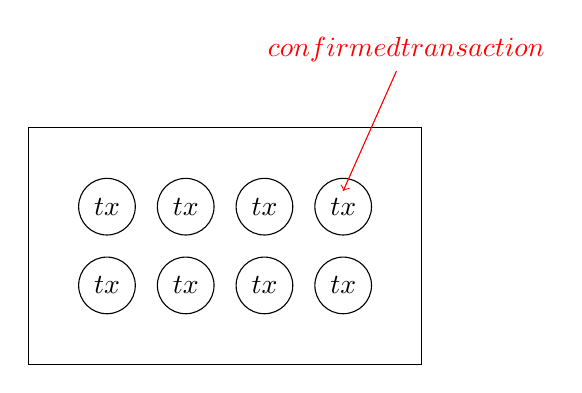
\begin{tikzpicture}
      \draw (0,0) rectangle (5,3);
      \foreach \x in {1,2,...,4}
        \foreach \y in {1,...,2}
          \node[circle,draw, minimum size=0.4cm] at (\x,\y) {$tx$};

      \node[red] (confirm) at (4.8, 4) {$confirmed \text{ }transaction$};
      \draw [->, red] (confirm) -- (4,2.2);
    \end{tikzpicture}
    \caption{A block}
    \label{fig:block:a}
  \end{subfigure}
  \begin{subfigure}[t]{0.40\textwidth}
    \centering
    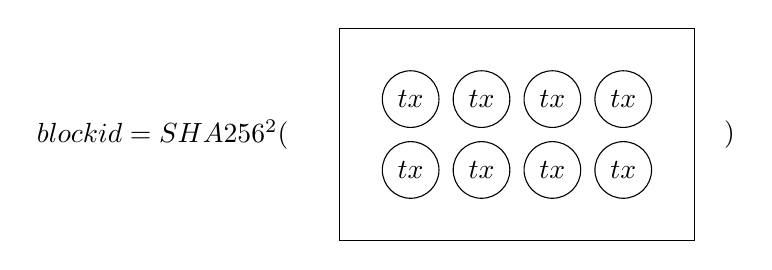
\begin{tikzpicture}[scale=0.9]
      \draw (0,0) rectangle (5,3);
      \foreach \x in {1,2,...,4}
        \foreach \y in {1,...,2}
          \node[circle,draw, minimum size=0.4cm] at (\x,\y) {$tx$};
      \node (txid) at (-2.5,1.5) {$blockid = SHA256^{2}($};
      \node (txid) at (5.5,1.5) {$)$};
    \end{tikzpicture}
    \caption{Bitcoin Block ID}
    \label{fig:block:b}
  \end{subfigure}
  \caption{Blocks}
  \label{fig:blocks}
\end{figure}

\begin{figure}[ht!]
  \centering
  \begin{tikzpicture}
    \foreach \x in {0,1,...,4}
        \pgfmathparse{(\x*3)}
        \edef\position{\pgfmathresult}
        \node[bl_block] (\x) at (\position,0) {$block$};

    \foreach \x in {1,2,...,4}
        \pgfmathparse{(\x-1)}
        \edef\previous{\pgfmathresult}
        \draw [->] (\x) -- (\previous);

  \end{tikzpicture}
  \caption{The blockchain}
  \label{fig:blockchain}
\end{figure}

\begin{figure}[ht!]
  \begin{tikzpicture}
    \foreach \x in {0,1,...,4}{
        \pgfmathparse{(\x*3)}
        \edef\position{\pgfmathresult}
        \node[bl_block] (\x) at (\position,0) {$block$};
        \pgfmathparse{int(\x*10 + 10)}
        \edef\time{\pgfmathresult}
        \node[] at (\position,-2) {$17:\time$};
    }


    \foreach \x in {1,2,...,4}
        \pgfmathparse{(\x-1)}
        \edef\previous{\pgfmathresult}
        \draw [->] (\x) -- (\previous);

    \node[ellipse, draw, red, inner xsep=6ex,inner ysep=3ex] (old_ell) at (0) {};
    \node[ellipse, draw, red, inner xsep=6ex,inner ysep=3ex] (recent_ell) at (4) {};
    \node[red,below=0cm of old_ell] (old) {$oldest\text{ }block\text{ }$};
    \node[red,below=0cm of recent_ell] (recent) {$recent\text{ }block\text{ }$};
  \end{tikzpicture}
  \caption{The blockchain timeline}
  \label{fig:blockchain_timeline}
\end{figure}

\section{Consensus mechanisms}\label{blockchain:consensus_mechanisms}

With the use of the blockchain data structure we manage to have a  chronological order of the transactions. What remains is a \textit{global agreement} on the order of the blocks among the participants of the network. Someone can easily change the order of two blocks within the chain by changing the respective hashes or producing new ones wherever required~\cite{zindros_thesis}. This would allow an adversary to fake the order of transactions in time, which is an undesired outcome.

The global agreement on a common truth, the global blockchain, is called \textit{consensus} -- a single universal “truth” -- and this is where Bitcoin's novelty is. The consensus mechanism is the core mechanism of the blockchain. Through consensus, the \textit{shared state} of the ledger comes to an agreement upon a global state, allowing all the nodes of the network to reach the same ledger state. That is, the users of the network agree on a common order of the blocks in the blockchain and therefore on the order of the transactions. Achieving consensus in a distributed system is challenging. A consensus mechanism has to be resilient to node failures, network delays and the existence of malicious nodes.

At high level, every public consensus mechanism works as follows: A ``game'', involving randomness, is taken place where each node of the network participates. The winner of the game is eligible to propose the new block that will be adopted in the blockchain. This is a simple, but a marvelous idea. The probabilistic nature of the process is paramount to its security~\cite{10.1007/978-3-662-46803-6_10}.

There are three basic consensus mechanism categories:

\begin{enumerate}
  \item Proof-of-Work (PoW).
  \item Proof-of-Stake (PoS).
  \item Practical Byzantine Fault Tolerance (PBFT)
\end{enumerate}


\subsection{Proof of Work (PoW)}\label{blockchain:consensus:pow}

A Proof-of-Work (PoW) consensus mechanism, is a consensus mechanism where each node of the network tries to solve a computational puzzle that is computational \textit{hard}, but feasible to find, and easy to verify \textit{correctness}. Assuming that hash functions are hard to invert, proof of work usually is established by seeking a range-collision of the hash function on the block~\cite{zindros_thesis}.

\begin{figure}[!ht]
  \centering
  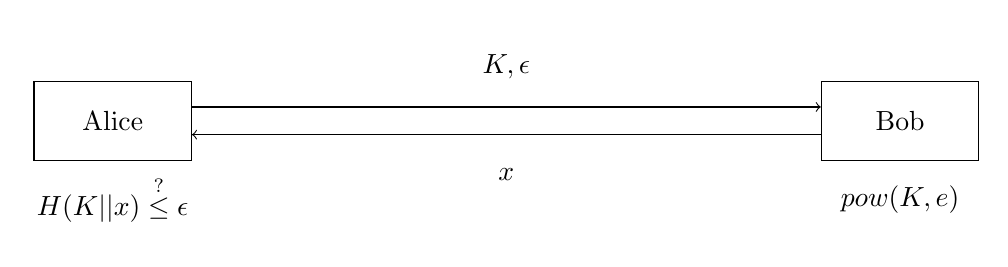
\begin{tikzpicture}[node distance=10cm, minimum height=1cm, minimum width=2cm]
    \node[draw] (a) {Alice};
    \node[draw, right of =a] (b) {Bob};
    \node[below of=a, node distance=1cm] (c) {$H(K || x) \stackrel{?}{\leq} \epsilon$};
    \node[below of=b, node distance=1cm] (d) {$pow(K, e)$};
    \draw[->] ([yshift=0.5em]a.east) -- ([yshift=0.5em]b.west) node[midway, above] {$K, \epsilon$};
    \draw[<-] ([yshift=-0.5em]a.east) -- ([yshift=-0.5em]b.west) node[midway, below] {$x$};
  \end{tikzpicture}
  \caption{The Proof-of-Work protocol}
  \label{fig:consensus:pow}
\end{figure}

Bitcoin~\cite{Zohar:2015:BUH:2817191.2701411} is the first blockchain system that utilizes a PoW for blockchain block generation. It work as follows: A \textit{target} $\epsilon$ is given and is asked that the hash of the block is \textit{smaller} than the target. The node can only modify a \textit{nonce}, which is concatenated with the rest of the block data. By changing the nonce the node can change the block hash. As cryptographic hash functions is assumed to be one-way, the only way to find a hash value smaller than the target is with a series of \textit{brute-force} trials of different nonce values. Bitcoin's proof-of-work can be summarized as:

\begin{equation*}
  H(txs || nonce || parent\_blockid) \leq \epsilon
\end{equation*}

The network evaluates collectively the target value using a predefined algorithm. That way, the network can control the difficulty of proof-of-work and the expected frequency of block generation is controlled. In Bitcoin the expected \textit{rate} is one block per 10 minutes.

All the nodes of the network simultaneously try to produce a new block, meaning trying to find a correct nonce satisfying the proof-of-work requirements. Each node monitors the network for blocks and transactions while preparing its block. In its block the node includes all the valid transactions that are not in a previous block and a reference to a parent block. Every node of the network can produce a valid block but each block has to meet the target proof-of-work requirements.

When a hash value less than the target is found by a node, the node gets to add the proposed block to the blockchain and broadcast the new block to all its neighbors which, in turn, transmit it to the whole network. If a block is found by another node, all the nodes stop the proof of work procedure and start over upon the new block. For a block to be accepted as valid it must contain valid transactions, a valid proof-of-work and a reference to a known valid parent block.

The existence of a transaction in a block makes the transaction valid. The deeper the block is in the blockchain the more difficult is for an adversary to alter the block in which the transaction is confirmed. The reason is, that the time an adversary needs to alter a block grows \textit{exponentially} in the number of blocks that have followed~\cite{10.1007/978-3-662-46803-6_10}, as she will need to reproduced those blocks and the blockchain is constantly extended. Waiting 6 confirmation blocks to appear after the block in which the transaction is confirmed is enough for a transaction to be considered secure.

A PoW system is based on \textit{randomness}. Each node has a small change to win the block which is approximated proportionally to the computational power of each node. The consensus mechanism depends on having a majority of the miners acting honestly out of self-interest~\cite{antonopoulos2014mastering}.

PoW consensus mechanism works very well in \textit{public} blockchain systems where trust of the nodes is low eliminating the double-spend problem and guarding against \textit{Sybil attacks}~\cite{sybil_attack}. However, the transaction confirmation time is longer compared to conventional financial services (such as VISA)~\cite{Sompolinsky2015,Zohar:2015:BUH:2817191.2701411,DBLP:journals/corr/abs-1708-05665} resulting in slower transaction confirmation rates. Lastly, the energy waste attributed to the mining process can be very high -- the energy requirements of the Bitcoin protocol are estimated to be comparable to those of a small country~\cite{6912770}.

\begin{lstlisting}[language=C, caption={A simple Proof-of-Work Algorithm}, mathescape=true]
  x = rand();

  do {
    ++x;
  } while (H(K||x) >= $\epsilon$);

  return x;
\end{lstlisting}

\subsection{Proof of Stake (PoS)}\label{blockchain:consensus:pos}

Proof-of-Stake algorithms are designed to overcome the disadvantages of PoW in terms of the high electricity consumption involved in mining~\cite{bl_consensus}
and provide equal security guarantees~\cite{Kiayias2017}. Unlike PoW where the nodes of the network solve computational puzzles in order to create a new block, in PoS the choice
of the block creator among the miners is random, yet relative to the \textit{stake} the node possesses according to the current blockchain ledger. Maintaining
the blockchain relies on the \textit{stakeholders} themselves and assigns work to them based on the amount of stake that each possesses as reported in the ledger~\cite{Kiayias2017}. The higher the stake participant, the higher the possibility to be chosen.

Proof-of-Stake algorithms suffer from the so-called `\textit{nothing at stake}' problem. The `nothing at stake' problem refers to attacks against PoS blockchain systems where shareholders do not have \textit{incentives} to follow the protocol and vote simultaneously on multiple blockchains exploiting the fact that little computational effort is needed to build a PoS blockchain~\cite{Kiayias2017}. Blockchains with PoS as a consensus mechanism can be either \textit{permissioned} or \textit{permissionless} in the sense of stake availability rather than node authorization. A node to participate in block election has to possess a stake. The market of stake has to be public and available for anyone for the network to be considered as truly permissionless. Otherwise, the initial stakeholders can sell stake selectively to participants of their choice making it permissioned. Ouroboros is the first \textit{provable} secure PoS algorithm~\cite{Kiayias2017} and is the main consensus algorithm of the Cardano blockchain~\cite{cardano_site}.

\subsection{Practical Byzantine Fault Tolerance (PBFT)}\label{blockchain:consensus:PBFT}

The \textit{Practical Byzantine Fault Tolerance} algorithm~\cite{Castro:1999:PBF:296806.296824} is the first practical consensus algorithm with Byzantine Fault Tolerance~\cite{byzantine_fault_tolerance}.
It is based on the concept of \textit{state machine replication} and \textit{replication state voting}, and is able to process tens of thousands of requests per second with minimal latency.
The algorithm has only a 3\% overhead over a typical filesystem~\cite{Castro:1999:PBF:296806.296824}.

PBFT and state-machine replication protocols’ downside is related to \textit{scalability}, in terms of the number of nodes (replicas)~\cite{Vukolić2016} that can be supported.
PBFT has only been scaled and studied up to 20 replicas~\cite{bl_consensus,Vukolić2016}. To overcome this limitation, without compromising security, various PBFT variants,
such as Ripple and Stellar, partition the network into smaller groups called federates and each one runs a local consensus protocol among its members and
global consensus is achieved when certain conditions are being met~\cite{DBLP:journals/corr/abs-1708-05665}.

\begin{table}[!ht]
  \centering
  \caption{Blockchain consensus mechanisms. Adapted and modified from~\cite{bl_consensus,Vukolić2016}}
  \begin{tabular}{|l|l|l|l|}
    \hline
    & PoW &	PoS &	PBFT \\ \hline
    Blockchain Type &	Permissionless &	Both &	Permissioned \\ \hline
    Scalability of nodes &	High &	High &	Low \\ \hline
    Scalability of clients &	High &	High &	High \\ \hline
    Transaction rate &	Low &	High &	High \\ \hline
    Latency &	High &	Low &	Minimal \\ \hline
    Power consumption &	High &	Low &	Low \\ \hline
    Token needed &	Yes &	Yes &	No \\ \hline
    Cost of participation &	Yes &	Yes &	No \\ \hline
  \end{tabular}
  \label{table:blockchain_consensus}
\end{table}

\section{Mining \& incentives}\label{blockchain:mining}

The process of creating a block in a PoW consensus system is known as \textit{mining} and the participants as \textit{miners}. The first block was mined by Satoshi Nakamoto~\cite{nakamoto2012bitcoin} and is called the \textit{genesis} block. Every valid chain starts from the genesis block.

For miners to participate in the network and contribute their computation resources incentives are provided. Normally, in permissionless blockchains such as Bitcoin or Ethereum a monetary incentive in the form of cryptocurrency incentivize the miners and in a permissioned blockchain finance incentives or access to blockchain data could encourage miners to participate~\cite{deloitte}.

In Bitcoin, the miner is rewarded with a number of bitcoins that are created for the specific block. This happens through a specific type of transaction called \textit{coinbase}. This type of transaction has an unconnected income edge without a sender and an outcoming edge with recipient the miner that found the particular block. This is how new bitcoins are generated. The amount of coin mined in each block is pre agreed by the network and every four years is reduced by half. Currently, the reward is 12,5 BTC.

\begin{figure}[!ht]
  \centering
  \begin{tikzpicture}
    \node[tx] (A) at (0,0) {$tx$};
    \draw [->] (-3,0) -- (A) node[midway, below]{} node[midway, above]{12.5 BTC};
    \draw [->] (A) -- (3, 0) node[midway, below]{miner} node[midway, above]{12.5 BTC};
  \end{tikzpicture}
  \caption{Coinbase transaction}
  \label{fig:mining:coinbase}
\end{figure}

Another way a miner is rewarded is by collecting \textit{transactions fees}; the financial remains of a confirmed transaction. This can happen when a user makes a transaction where the total value of all incoming edges are bigger than the total value of all outcoming edges. In particular, the total fees of a block are defined as:

\begin{equation*}
  fees = \sum_{tx \in block} [ \sum_{i \in in(tx) }w(i) -  \sum_{o \in out(tx) }w(o)]
\end{equation*}

\section{Blockchain fork}\label{blockchain:fork}

Due to network latency and the distributed nature of the system, it is possible that two miners will find a block around the same time and some nodes will accept the first block and some others the second one. Both blocks are valid, containing a valid proof of work, valid transactions and both extent the same parent block. In such cases there is a temporary \textit{fork} in the blockchain, where some nodes are adding blocks to one branch while other nodes are adding blocks to another branch. As a result, two competitive versions of the blockchain will emerge~\cite{antonopoulos2014mastering}. Similarly to transactions, the order of the blocks cannot be defined.

To resolve this, each node always selects the longest brach. At some point, one of the two branches will be extended by a new block. The nodes that were working on the first branch will see that the new branch is the longest and start working immediately on that. Eventually the system will come to an agreement, the longest branch will be accepted and the others will be discarded. The process of chain selection can be likened to voting where mining nodes ``\textit{vote}'' with their mining power by choosing which chain to extend by mining the next block; the new block itself represents the voting result~\cite{antonopoulos2014mastering}.

\begin{figure}[!ht]
  \centering
  \begin{tikzpicture}
    \foreach \x in {0,1,...,5}
        \pgfmathparse{(\x*2)}
        \edef\position{\pgfmathresult}
        \node[bl_block, minimum width=1cm, fill=blue!30] (\x) at (\position,0) {$block$};

    \foreach \x in {1,2,...,5}
        \pgfmathparse{(\x-1)}
        \edef\previous{\pgfmathresult}
        \draw [->] (\x) -- (\previous);

    \foreach \x in {3,4}
        \pgfmathparse{(\x*2)}
        \edef\position{\pgfmathresult}
        \node[bl_block, minimum width=1cm, fill=orange!30] (\x_fork) at (\position,2) {$block$};

    \draw [->] (4_fork) -- (3_fork);
    \draw [<-] (2.north) -- (3_fork.west);

  \end{tikzpicture}
  \caption{A blockchain fork}
  \label{fig:bl:fork}
\end{figure}

If a malicious adversary wants to do create double spent transactions or execute a denial-of-service, she has to produce a malicious blockchain \textit{longer} than the honest. To achieve that, an adversary would need to control the majority of the CPU power of the network and specifically more than 51\% of the total network’s hashing power. This is called the \textit{51\% attack}. It is important to node that this kind of consensus attack affects at best the most recent blocks. Beyond a certain depth blockchain is absolute immutable. In addition, this type of attacks cannot steal or spend coins as the adversary has to forge a signature to produce a valid transaction impersonating another user. Bitcoin's security has been formalized and rigorously explored~\cite{10.1007/978-3-662-46803-6_10} over the last years.

 Ethereum is designed to produce blocks very fast (around 12-15 second) in comparison to Bitcoin (around 10 minutes). Blockchains with fast block confirmation times, suffer from reduced security due to high \textit{stale rate}~\cite{ethereum_whitepaper}. To counterpart that, Ethereum use a variant of the \textit{GHOST} protocol~\cite{Sompolinsky2015}. The GHOST protocol rule picks the chain that has had the \textit{most computation} done upon it and not the chain with the longest depth. It takes into account all stale blocks of the chain including all stale descendants of the block's ancestor.

\begin{figure}[ht!]
  \centering
  \begin{tikzpicture}
    \foreach \x in {0,1,...,5}
        \pgfmathparse{(\x*2)}
        \edef\position{\pgfmathresult}
        \node[bl_block, minimum width=1cm, fill=blue!30] (\x) at (\position,0) {};

    \foreach \x in {1,2,...,5}
        \pgfmathparse{(\x-1)}
        \edef\previous{\pgfmathresult}
        \draw [->] (\x) -- (\previous);

    \foreach \x in {3,...,6}
        \pgfmathparse{(\x*2)}
        \edef\position{\pgfmathresult}
        \node[bl_block, minimum width=1cm, fill=red!30] (\x_mal) at (\position,2) {};

    \draw [->] (4_mal) -- (3_mal);
    \draw [->] (5_mal) -- (4_mal);
    \draw [->] (6_mal) -- (5_mal);

    \draw [<-] (2.north) -- (3_mal.west);

    \node[circle, draw, minimum size=0.1cm, fill=red] at (4_mal.center) {};
    \node[circle, draw, minimum size=0.1cm, fill=green] at (3.center) {};

    \draw[decorate,decoration={brace,amplitude=10pt, mirror}, xshift=-1.2em, yshift=-1.5em](0, 0) -- (5, 0) node [black,midway,yshift=-1cm, above] {\footnotesize{Honest common prefix}};

    \draw[decorate,decoration={brace,amplitude=10pt, mirror}, xshift=-1.2em, yshift=-1.5em](6, 0) -- (11, 0) node [black,midway,yshift=-1cm, above] {\footnotesize{Honest blockchain}};

    \draw[decorate,decoration={brace,amplitude=10pt}, xshift=-1.2em, yshift=1.5em](6, 2) -- (13, 2) node [black,midway, above, yshift=1em] {\footnotesize{Malicious blockchain}};

  \end{tikzpicture}
  \caption{Double spent attack}
  \label{fig:blockchain:dl_spent}
\end{figure}

\section{Blockchain Types}\label{blockchain:blockchain_types}

There are various types of blockchains varying in restrictions on data access and participation in the consensus process. Each one has its own advantages and disadvantages.

\begin{itemize}
  \item \textbf{Public Blockchain}: A public blockchain is a blockchain, in which there are no restrictions on reading blockchain data--encrypted or not--and validating transactions~\cite{prbc_vs_pubbc}.
  The most common implementation of a public blockchain is Bitcoin~\cite{nakamoto2012bitcoin} and Ethereum~\cite{ethash}.
  \item \textbf{Federated or Consortium blockchain}: In a federated blockchain transaction validation is limited to a predefined list of entities with their identities known to the network. Data access can either be public or restricted~\cite{prbc_vs_pubbc}.
  \item \textbf{Private blockchain}: A private blockchain is a blockchain where consensus mechanism is centralized to one single entity regardless of data access~\cite{prbc_vs_pubbc}.
\end{itemize}

\section{Consensus defined types of Blockchain}\label{blockchain:consensus_blockchain_types}

\begin{itemize}
  \item \textbf{Permissionless blockchain}: A permissionless blockchain is a blockchain, in which there are no restrictions on identities of transaction processors (i.e., users that are eligible to create blocks of transactions)~\cite{prbc_vs_pubbc}.
  \item \textbf{Permissioned blockchain}: A permissioned blockchain is a blockchain, in which transaction processing is performed by a predefined list of subjects with known identities~\cite{prbc_vs_pubbc}.
\end{itemize}

\begin{table}[!ht]
  \centering
  \caption{Blockchain Types. Source~\cite{hub-bl-types}}
  \begin{tabular}{|l|l|l|l|}
    \hline
     & Public & \makecell[cl]{Permissioned \\ (Multiple Entities)} & \makecell[cl]{Private \\ (Single Entity)} \\ \hline
     Participants & \makecell[cl]{Permissionless \\ Anonymous} & \makecell[cl]{Permissioned \\ Identified \\ Trusted} & \makecell[cl]{Permissioned \\ Identified \\ Trusted} \\ \hline
     Data Access & Public & Public or Restricted & Restricted \\ \hline
     Consensus & PoW, PoS & FBTA, PoS & FBTA \\ \hline
  \end{tabular}
  \label{table:blockchain_types}
\end{table}

\section{Smart Contracts}
\label{smart_contracts}

A \textit{smart contract} is a computer protocol intended to facilitate, verify, or enforce the negotiation or performance of a contract~\cite{FM548,szabo1996smart}.
The idea of smart contracts proposed in the early 1990s~\cite{FM548}, by Nick Szabo, and have been used primarily in association with cryptocurrencies enabling
parties to formally specify a cryptographically enforceable agreements~\cite{7163021}. A smart contract consists of a set of promises including protocols within which the parties perform on these promises. It can define rules and penalties around an agreement and automatically enforce those obligations. The contractual rules may be partially or fully self-executed, self-enforcing or both. On blockchain technologies a smart contract is any computer program that is executed on the blockchain -- a general purpose computation.

\subsection{Bitcoin scripts}
\label{smart_contracts:bitcoin}

Bitcoin is the first blockchain that provides a \textit{scripting} language for expressing simple smart contracts such as ownership of an amount of coins by one or multiple entities. Bitcoin's language is a \textit{stack-based} scripting language inspired by Forth~\cite{forth_lang} and offers a set of simple \textit{serial commands} supporting cryptographic primitives such as hash functions and signature verification. The main disadvantage of Bitcoin's language is that is not \textit{Turing-complete} limiting the type of smart contracts one can create. Furthermore, adding new commands to extent functionality requires either a soft-fork which has to be decided by the majority of bitcoin network or to fork Bitcoin's code and implement a new blockchain supporting the new features in which the Bitcoin's network power is lost. Numerous previous smart contract application atop Bitcoin (e.g., lottery\cite{Andrychowicz:2014:SMC:2650286.2650764,10.1007/978-3-662-44381-1_24}, verifiable computation~\cite{Kumaresan:2014:UBI:2660267.2660380}) have demonstrated the difficulty of Bitcoin's scripting language~\cite{cryptoeprint:2015:675}.

In~\ref{blockchain:structure:tx}, a transaction is defined as a graph node with two edges, one incoming and one outcoming and each edge has an owner declared by her address. In reality, each edge contains a program which decides whether the edge can be spent or not. The program is written in Bitcoin's scripting language and is called \verb|scriptPubKey|. This allows the expression of more complicated ownership of assets such as \textit{multi-signatures} or \textit{micropayments}. The script is executed on a stack machine and containes a series of simple serial commands. When a UTXO is spent, every node of the network executes the \textit{script}. If the output of the program is $1$, then the transaction is valid and can be spent. Otherwise, the transaction is considered invalid.

\begin{figure}[!ht]
  \centering
  \begin{tikzpicture}
    \node[tx] (A) at (0,0) {$tx$};
    \draw [->] ++(-8,0) -- (A) node[above, midway]{5mBTC} node[left, below,  align=left, font=\footnotesize, xshift=-4.5cm]{
      OP\_DUP \\
      OP\_HASH160 \\
      1FdtUtvK5vZxwo8jzjzid5EwGAB7paqX4n \\
      OP\_EQUALVERIFY \\
      OP\_CHECKSIG
    };
    \draw [->] (A) -- (8, 0) node[midway, above]{5mBTC} node[midway, below, align=left, font=\footnotesize, xshift=0.2cm]{
      OP\_DUP \\
      OP\_HASH160 \\
      128MZKqUsvg2kYJQ5LCVDx8Mdn8xrijzQY \\
      OP\_EQUALVERIFY \\
      OP\_CHECKSIG};
  \end{tikzpicture}
  \caption{A Bitcoin script}
  \label{fig:bl_tx:script}
\end{figure}

\subsection{Ethereum smart contracts}
\label{smart_contracts:ethereum}

The need of user defined open source blockchain applications emerged. As a result, \textit{Ethereum}~\cite{ethereum_yellowpaper, ethereum_whitepaper} was born. Ethereum is an open-source, public, blockchain-based distributed computing platform and a smart contract framework that enables anyone to build \textit{distributed applications} making the process much easier and efficient than ever before. It provides a decentralized Turing-complete virtual machine, the \textit{Ethereum Virtual Machine} (EVM) in which smart contracts are executed by all nodes of the network. In Ethereum, one can create smart contracts in a high level language, such as \textit{Solidity}~\cite{solidity}, which in turn is compiled to \textit{bytecode} that is executable on the EVM. Ethereum provides a cryptocurrency called \textit{Ether} which can be transferred between accounts, and \textit{gas}, an internal pricing mechanism used to execute contracts and allocate resources on the network. Like Bitcoin, Ethereum use a Proof-of-Work consensus mechanism called \textit{Ethash} and has been designed to be \textit{ASIC-resistant}~\cite{ethash}. Soon Ethereum will be moved to a Proof-of-Stake consensus mechanism called \textit{Casper}.

With Ethereum launch, the notion of \textit{DApps} (decentralized applications) arisen
and a lot of developers and companies are building numerous applications atop Ethereum such as prediction markets~\cite{augur,gnosis}, social media platforms~\cite{akasha,backfeed},
online gambling~\cite{etheroll,coinpoker} and video games~\cite{cryptokitties}. As of January 2018, there are more than 250 live DApps.

Before describing how smart contracts are deployed in Ethereum, a thorough analysis of Ethereum's core mechanisms must be made. Ethereum constitute of a set of one global object, that of \textit{account}. Each account has a \textit{state}, in which the nodes of the network must agree upon with the use of a consensus mechanism, and a 20-byte address. The state of an account can only be changed by a transaction. The global state of Ethereum is made up of accounts. For that reason, Ethereum is often described as a \textit{state machine}~\cite{ethereum_whitepaper} where the \textit{state transition function} takes as input a transaction and outputs a different state.

Each account is composed by the following fields: \textit{address}, \textit{balance}, and \textit{nonce}. The address is a 160-bit account identifier which corresponds to a public key. The balance contains the total amount the account holds in \textit{Wei}; the smallest denomination of ether. Ethereum instead of using UTXOs to keep track of coin ownership, adopted the traditional notion of balances for which we are accustomed from the financial system. The choice of balances over UTXOs was a design decision by the Ethereum foundation. Each option has its advantages and disadvantage. According to Ethereum founders, the advantages of accounts massively outweigh the alternatives~\cite{eth_design}. Lastly, the nonce is the total number of transaction sent from that account and it acts as a \textit{replay-attack} prevention mechanism. A malicious adversary could hear a transaction and broadcast a copy of it in another time. As a result, the transaction amount will be deducted again from the user's balance since the transaction is valid.

Similar to Bitcoin, anyone can send ethers from one account to another. The principles of the transaction described in~\ref{blockchain:structure:tx} are also applicable to Ethereum. Each transaction consist of the following fields: \textit{from}, \textit{signature}, to, and \textit{amount}. The from and to fields describe the sender and the receiver respectively. The signature field contains the valid signature of the transaction where the nodes of the network verify. Lastly, the amount contains the amount to be sent in Wei.

There are two type of accounts: \textit{personal} (or external own accounts) and \textit{contract} accounts. A contact account is an account dedicated for smart contracts. They contain two extra fields: \textit{code} and \textit{storage}. The code field contains the code of the smart contract and the storage field the internal persistent storage of the smart contract. Those fields are empty, and optional, when it comes to personal accounts.

\begin{figure}[!ht]
  \centering
  \begin{tikzpicture}[x=2cm, y=-1cm, node distance=0 cm,outer sep = 0pt]
    \node[account_block, fill=orange!30] (address) {$address$};
    \node[account_block, right=of address, fill=magenta!30] (code) {$code$};
    \node[account_block, right=of code, fill=purple!30] (storage) {$storage$};
    \node[account_block, right=of storage, fill=blue!30] (balance) {$balance$};
    \node[account_block, right=of balance, fill=green!30] (nonce) {$nonce$};
  \end{tikzpicture}
  \caption{An Ethereum account}
  \label{fig:eth_account}
\end{figure}

Additionally, transactions contain also an extra field, called \textit{data} field. To create a contact, a transaction with empty recipient and in data field the code of the smart contract must be created and sent. When the nodes of the network hear a transaction, where the field of the recipient is empty, they treat the transaction as a smart contract creation transaction. They create a contract account with code, the string that is contained in the data field of the transaction, and empty storage. After the creation of the contract account an address is returned to the creator of the contract. The address is created from the concatenation of the creator's public key and her account current nonce. Anyone knowing the address of the contract can interact with it. In particular, to call a smart contract function, a transaction with recipient the smart contact's address and data the function's name along with its arguments, has to be sent.

\begin{table}[!ht]
  \centering
  \caption{Ethereum accounts}
  \begin{tabular}{|c|c|c|}
  \hline
   & Personal account  & Contract account \\ \hline
   address & $H(p_k)$ & $H(creator, nonce)$ \\ \hline
   code & $\emptyset$ & Code to be executed \\ \hline
   storage & $\emptyset$ & Data of the contract \\ \hline
   balance & \multicolumn{2}{c|}{ETH} \\ \hline
   nonce &  \multicolumn{2}{c|}{\# transaction sent}  \\ \hline
  \end{tabular}
  \label{fig:eth_accounts}
\end{table}

When a contract account is activated, the contract code runs and it can read or write to internal storage, do various computations, send messages or create new contracts. A contract account can not initiate new transactions on its own but only in response of a transaction initiated by a personal account. Only personal accounts can change the state of the accounts.

Contract accounts can send \textit{messages} to other contracts accounts. Messages are like transactions except it is produced by a contract and exist only in the Ethereum execution environment. The network never sees the message neither is stored in the blockchain. This way, contracts can have relationships with other contracts.

\begin{table}[!ht]
  \centering
  \caption{Ethereum transactions}
  \begin{tabular}{|c|c|c|c|}
  \hline
   & create & send & call \\ \hline
   from & creator & sender & caller \\ \hline
   signature & $\sigma$ & $\sigma$ & $\sigma$ \\ \hline
   to & $\emptyset$ & receiver & contract \\ \hline
   amount & \multicolumn{3}{c|}{ETH} \\ \hline
   data & code & $\emptyset$ & $f, args$ \\ \hline
  \end{tabular}
  \label{fig:eth_transactions}
\end{table}

\begin{figure}[!ht]
  \centering
  \begin{tikzpicture}[scale=0.5, node distance=2.5 cm,outer sep = 0pt]
    \node[node, fill=blue!30] (pr_1) {Personal Account};
    \node[node, fill=blue!30, below=of pr_1] (pr_2) {Personal Account};
    \node[node, fill=orange!30, right=of pr_1] (c_1) {Contract Account};
    \node[node, fill=orange!30, below=of c_1] (c_2) {Contract Account};
    \node[node, fill=orange!30, right=of c_2] (c_3) {Contract Account};

      \draw [->] (pr_1) -- (c_1);
      \draw [->] (pr_2) -- (c_2);
      \draw [->] (c_1) -- (c_2);
      \draw [->] (c_2) -- (c_3);
  \end{tikzpicture}
  \caption{Transactions \& messages}
  \label{fig:eth_transaction}
\end{figure}

When a transaction call a function of a contract, the code of that function is run by all nodes of the network. The function can change the state of the contract or the state of another account. The nodes must agree on a global common state for that account. Similar to Bitcoin, the transactions, along with the state of each account, are contained in a block which through a proof-of-work consensus mechanism the network agree upon the block that will extent the blockchain and consequently to the new state of the accounts.

As all nodes evaluate all transactions, execute code and store all state, and the Ethereum is turing-complete, infinite loops or computational heavy code could make all the nodes of the system to be occupied for a very long period of time, or even forever, and any other transactions waiting for validation will not be fulfilled. Furthermore, storage requirements can be grown very fast making the nodes to become unable to fulfil and maintain that demand as there is no incentive to invest for storage capacity. To address those issues, Ethreuem use a unit called \textit{gas} as a measurement of computation use. It acts as a anti-denial of service mechanism. The intent of the gas, is that a malicious adversary should pay proportionately for every resource that they consume, including computation, bandwidth and storage~\cite{ethereum_whitepaper}.

So, gas is an internal pricing mechanism used to execute contracts and allocate resources on the network and it's price is expressed in \textit{gwei} ($1 \times 10^9$ Wei). Every node in the Ethereum network executes instructions (\textit{opcodes}), that represent the code of the contract, within the Ethereum Virtual Machine (EVM) and each of these instructions has an associated cost in gas. The cumulative sum of all the operations is the total gas cost for a transaction and is the fee that is being paid to the miners.

The cost of each opcode (operation code) of EVM is defined in Ethereum's yellow paper~\cite{ethereum_yellowpaper} and a gas cost summarization of basic opcodes are be shown in Table~\ref{table:opcode_gas_cost}. For storing data, Ethereum offers two opcodes: the \textit{SLOAD} opcode which loads a word from the storage and the \textit{SSTORE} opcode which saves a word to storage. The size of an EVM word is 32 bytes (256 bit) and to store one EVM word using the SSTORE opcode costs 20.000 gas. Due to that reasons, storing data is expensive and for the moment blockchain technologies cannot be used for file saving or dig data processing.

\begin{table}[!ht]
  \centering
  \caption{Ethereum opcodes gas costs}
  \begin{tabular}{|l|l|l|}
  \hline
   Operation & Gas  & Description \\ \hline
   ADD/SUB & 3 & Arithmetic operation \\ \hline
   MUL/DIV & 5 & Arithmetic operation \\ \hline
   ADDMOD/MULMOD & 8 & Arithmetic operation \\ \hline
   AND/OR/XOR & 3 & Bitwise logic operation \\ \hline
   LT/GT/SLT/SGT/EQ & 3 & Comparison operation \\ \hline
   POP & 2 & Stack operation \\ \hline
   PUSH/DUP/SWAP & 3 & Stack operation \\ \hline
   MLOAD/MSTORE & 3 & Memory operation \\ \hline
   JUMP & 8 & Unconditional jump \\ \hline
   JUMPI & 10 & Conditional jump \\ \hline
   SLOAD & 200 & Storage operation \\ \hline
   SSTORE & 5.000 / 20.000 & Storage operation \\ \hline
   BALANCE & 400 & Get balance of an account \\ \hline
   CREATE & 32.000 & Create a new account using CREATE \\ \hline
   CALL & 25.000 & Create a new account using CALL \\ \hline
   LOG & 375 & Logging operation \\ \hline
  \end{tabular}
  \label{table:opcode_gas_cost}
\end{table}

An Ethereum transaction has two extra fields: the \textit{start gas} and \textit{gas price}. The start gas is the maximum amount of gas willing to pay and the gas price is the price willing to pay per gas unit. The start gas (or gas limit) acts as a protection to computational wastage or malicious code. Even if the code needs more gas to terminate, when the gas limit is reached the execution is stoped and all state changes are revert. An extra benefit of gas limit is, that a miner seeing the gas limit field can estimate the needed computational time beforehand and act accordingly. The gas price is not defined by any central trusted authority but is regulated by the network itself. By setting the gas price, the user in a sense ``votes'' for the value of the gas. Gas price determines how quickly a transaction will be mined; the higher the price is, the more likely is the transaction to be in the next block.

\begin{figure}[!ht]
  \centering
  \begin{tikzpicture}[x=2cm, y=-1cm, node distance=0 cm,outer sep = 0pt]
    \node[account_block, fill=orange!30] (from) {$from$};
    \node[account_block, right=of from, fill=magenta!30] (signature) {$signature$};
    \node[account_block, right=of signature, fill=purple!30] (to) {$to$};
    \node[account_block, right=of to, fill=blue!30] (amount) {$amount$};
    \node[account_block, right=of amount, fill=green!30] (data) {$data$};
    \node[account_block, right=of data, fill=yellow!30] (startgas) {$startgas$};
    \node[account_block, right=of startgas, fill=blue!30] (gasprice) {$gasprice$};
  \end{tikzpicture}
  \caption{An Ethereum transaction}
  \label{fig:eth_transaction}
\end{figure}

The start gas can be larger than the cost of the computation. In this case, all unused gas is refunded at the end of a transaction to the sender. If the computation exceed the gas limit then a \textit{out of gas exception} is triggered and the state is reverted to the previous one. Out of gas exceptions are not refundable. The miner still claims the fee for each computational step performed.

\begin{figure}[!ht]
  \begin{tikzpicture}[node distance=2.5cm]
    \node[execution_entity, label=below:{\footnotesize{250}}] (sender) at (0, 0) {Sender};
    \node[execution_process, right =of sender] (start) {Start \\ Transaction};
    \node[execution_operation, right =of start, label=below:{\footnotesize{200}}] (op_1) {Operation};
    \node[execution_operation, right =of op_1, label=below:{\footnotesize{170}}] (op_2) {Operation};
    \node[execution_process, below =of start, label=below:{\footnotesize{170}}] (end) {End \\ Transaction};
    \node[execution_entity, right =of end] (receiver) {Receiver};

    \node[execution_label, below=of end] (rem_gas) {Remaing \\ gas};
    \node[execution_label, below=of sender] (str_gas) {Start \\ gas};

    \draw[->] (sender) -- (start);
    \draw[->] (start) -- (op_1) node[midway, above, red]{\footnotesize{Use -50 gas}};
    \draw[->] (op_1) -- (op_2) node[midway, above, red]{\footnotesize{Use -30 gas}};
    \draw[->] (op_2.east) -- ++(0.5, 0) -- ++(0, -1.5) -- ++(-11.4, 0) -- (end.north);
    \draw[->] (end) -- (receiver);

    \draw[->] ([yshift=-0.55cm]end.south) -- (rem_gas);
    \draw[->] (rem_gas.west) -- ++(-4.2, 0) -- (str_gas);

    \draw[<-] ([yshift=-0.55cm]sender.south) -- (str_gas);
  \end{tikzpicture}
  \caption{Smart contract execution}
  \label{fig:smart_contract_execution}
\end{figure}

\begin{figure}[!ht]
  \begin{tikzpicture}[node distance=2.5cm]
    \node[execution_entity, label=below:{\footnotesize{250}}] (sender) at (0, 0) {Sender};
    \node[execution_process, right =of sender] (start) {Start \\ Transaction};
    \node[execution_operation, right =of start, label=below:{\footnotesize{200}}] (op_1) {Operation};
    \node[execution_operation, right =of op_1, label=below:{\footnotesize{170}}] (op_2) {Operation};

    \node[execution_operation, below =of op_2, label=below:{\footnotesize{0}}] (op_3) {Operation};
    \node[execution_operation, left =of op_3, label=below:{\footnotesize{0}}] (op_4) {Operation};

    \node[execution_entity, below =of op_3] (receiver) {Receiver};

    \node[execution_label, below=of sender] (str_gas) {Start \\ gas};

    \draw[->] (sender) -- (start);
    \draw[->] (start) -- (op_1) node[midway, above, red]{\footnotesize{Use -50 gas}};
    \draw[->] (op_1) -- (op_2) node[midway, above, red]{\footnotesize{Use -30 gas}};
    \draw[->] ([yshift=-0.55cm]op_2.south) -- (op_3) node[midway, left, red]{\footnotesize{Use -170 gas}};
    \draw[->] (op_3) -- (op_4) node[midway, above, red]{\footnotesize{Out of gas}};

    \draw[red!100, thick] ([yshift=1cm]sender |- receiver.north) -- ([yshift=1cm]receiver.north) node[midway, below, red]{\footnotesize{Revert state}};

    \draw[<-] ([yshift=-0.55cm]sender.south) -- (str_gas);
  \end{tikzpicture}
  \caption{Out of gas exception}
  \label{fig:smart_contract_out_of_gas}
\end{figure}

Each miner at code execution perform the following steps:

\begin{enumerate}
  \item If $start\_gas * gas\_price > balance$ then halt
  \item Deduct $start\_gas * gas\_price$ from $balance$
  \item Set $gas = start\_gas$
  \item Run code deducting from gas
  \item After termination return remaining $gas$ to $balance$
\end{enumerate}

The total gas cost of the transaction is paid to miner that mined the block. The \textit{maximum fee} a miner could take by a transaction is calculated as:

\begin{equation*}
  fee_{max} = startgas \times gasprice
\end{equation*}

For example if the start gas is set to $50.000$ and the gas price to $20$ Gwei the maximum fee is $0.001$ ETH.

As discussed earlier, the code of the contract is executed within the Ethereum Virtual Machine (EVM) which is a stack-based machine using 32-bytes (256-bit) words. The EVM is a virtual machine that reads a series of bytecode instructions (EVM code) where each bytecode represents an operation (opcode). In addition, EVM provides built-in cryptographic primitives support.

\begin{lstlisting}[language=Solidity, caption={EVM bytecode}]
PUSH1 0
CALLDATALOAD
SLOAD
NOT
PUSH1 9
JUMPI
STOP
JUMPDEST
PUSH1 32
CALLDATALOAD
PUSH1 0
CALLDATALOAD
SSTORE
\end{lstlisting}

Writing smart contract on bytecode can be challenging. For that reason, various high level programming language that compile to EVM code have been implemented. The most wide used is Solidity~\cite{solidity}. From the perspective of a developer, Solidity is much alike to JavaScript as it supports most of its structures. Every contact have to be declared with the keyword \verb|contract| at the begging of the file. It is the same as declaring a class or an object in object-oriented programming languages.

Solidity supports two types of variables: \textit{state} variables and \textit{local} variables. State variables are contract variables that are permanently stored in contract storage and have to be declared at compilation time. Local variables are function variables that cannot be accessed outside the scope of the function and they can be stored either in storage or memory. Without declaration, local variables of \verb|struct|, \verb|array| or \verb|mapping| type reference are saved in storage by default and local variables of value type are stored in the stack.

The value types of variables Solidity supports are:

\begin{itemize}
  \item Boolean: true of false.
  \item Integers: Signed and unsigned integers of various sizes. Keywords \verb|uint8| to \verb|uint256| in steps of  8 (unsigned of 8 up to 256 bits) and \verb|int8| to  \verb|int256|.
  \item Fixed-size byte arrays: \verb|bytes1| to  \verb|bytes32| in steps of one.
  \item Dynamically-sized byte array: \verb|bytes| or \verb|string|.
  \item Address: 20-byte value holding an Ethereum address.
  \item Enum: Enumerated type.
  \item Mapping: A key-map type similar to hash tables. \verb|mapping(keyType => valueType)|.
  \item Structs: A structure. It can be used to define new types.
  \item Function: Variables that hold a function reference.
\end{itemize}

EVM supports a built-in logging mechanism which can be used by smart contracts to notify various events. Services outside the blockchain can register listeners to those event and act accordingly; log and event data is not accessible from within contracts~\cite{solidity}. As logging events is much cheaper than saving data to storage, the log is often used as an alternative to store data cheaply; a LOG opcode costs 375 gas and for each byte of data it costs 8 gas, way lower than SSTORE opcode. In solidity, an event is declared by the \verb|event| keyword along with its arguments. Lastly, Solidity supports multiple inheritance including abstract class and interfaces. Contracts can extend another contract with the keyword \verb|is| and access internal functions and non-private members.

Since smart contracts deal directly with currency exchange, security of smart contract is of the utmost importance~\cite{safe_smart_contracts, smart_contracts_smarter}. The DAO bug~\cite{dao, dao_2} is a perfect example where at least 60 millions US dollars was lost leading to a hard fork in Ethereum and the creation of Ethereum Classic. In contrast to traditional application that can be patched when bugs are detect, smart contracts, due to the nature of blockchain, are irreversible and immutable. Various analysis~\cite{safe_smart_contracts, smart_contracts_smarter} have shown that most of the deployed smart contracts on Ethereum are vulnerable. In particular, an analysis tool called \verb|Oyente|~\cite{smart_contracts_smarter}, created by Loi Luu et. al, marked 8,833 out of 19,336 smart contracts as vulnerable. Is believed that these bugs arise from the gap in understanding the actual mechanisms of the underlying platform of Ethereum~\cite{smart_contracts_smarter}; developers make false assumptions of the semantics of the system.

\subsection{Cardano}\label{blockchain:impl:cardano}

Another platform for smart contract implementation is Cardano. Cardano is a security focused blockchain that utilize the latest research and engineering insights to build a platform suitable for the highest value applications~\cite{cardano_site}. It supports distributed applications creation and smart contracts verifiable by a method called formal verification allowing logical proof of correctness of code providing high security. Cardano addresses the need for regulatory oversight while maintaining consumer privacy and security. Cardano is the first blockchain project to be peer reviewed by academic researchers~\cite{cardano_site} and its consensus mechanism, \textit{Ouroboros}, is the first Proof of Stake algorithm to be provably secure~\cite{Kiayias2017}. Cardano consists of two main layers, one for accounting and one for computation. The accounting layer is called \textit{Cardano Settlement Layer} (CSL)
and the computation layer \textit{Cardano Computation Layer} (CCP) where distributed application can be built and run upon. The CCP layer has not been implemented yet and there is a plan to be released as a beta by the first quarter of 2018~\cite{cardano_parsons}.

\clearpage

\begin{lstlisting}[language=Solidity, caption={An Ethereum Smart Contract}]
pragma solidity ^0.4.16;

contract Namespace{

  struct NameEntry {
      address owner;
  }

  uint32 constant REGISTRATION_COST = 100;
  uint32 constant UPDATE_COST = 10;
  mapping(bytes32 => NameEntry) data;

  function nameNew(bytes32 hash){
      if (msg.value >= REGISTRATION_COST){
          data[hash].owner = msg.sender;
      }
  }

  function nameUpdate(bytes32 name, bytes32 newValue, address newOwner){
      bytes32 hash = sha3(name);
      if (data[hash].owner == msg.sender && msg.value >= UPDATE_COST) {
          data[hash].value = newValue;
          if(newOwner != 0) {
              data[hash].owner = newOwner;
          }
      }
  }

  function nameLookup (bytes32 name) {
      return data[sha3(name)]
  }
}
\end{lstlisting}

\clearpage
